\documentclass[conference]{IEEEtran}






% *** GRAPHICS RELATED PACKAGES ***
%
\ifCLASSINFOpdf
\usepackage[pdftex]{graphicx}
\graphicspath{{images/}}
  % declare the path(s) where your graphic files are
  % \graphicspath{{../pdf/}{../jpeg/}}
  % and their extensions so you won't have to specify these with
  % every instance of \includegraphics
  % \DeclareGraphicsExtensions{.pdf,.jpeg,.png}
\else
  % or other class option (dvipsone, dvipdf, if not using dvips). graphicx
  % will default to the driver specified in the system graphics.cfg if no
  % driver is specified.
  % \usepackage[dvips]{graphicx}
  % declare the path(s) where your graphic files are
  % \graphicspath{{../eps/}}
  % and their extensions so you won't have to specify these with
  % every instance of \includegraphics
  % \DeclareGraphicsExtensions{.eps}
\fi


% correct bad hyphenation here
\hyphenation{op-tical net-works semi-conduc-tor}


\begin{document}

\title{K.I. für Hilfsmittel für Angreifer}

\author{\IEEEauthorblockN{Dominik Kaier}
\and
\IEEEauthorblockN{Timo Max}
\and
\IEEEauthorblockN{Henrik Busch}}

\maketitle

\begin{abstract}
Diese Ausarbeitung zeigt den Stand der Technik von K.I. im Cyber Sicherheitsbereich für Angreifer. Dazu wird auf die drei Angriffsvektoren: Phishing \& Socialengineering, Code Schwachstellenanalyse \& Exploit generierung, Physische Schwachstellenanalyse \& Exploit generierung eingegnagen. Im Vergleich Mythos vs öffentliche Modelle wird klar das es kein exklusiv Werkzeug ist.
\end{abstract}

\include{chapters/chapter1}

\IEEEpeerreviewmaketitle



\section{Einführung}
Im April 2026 wurde das LLM-Modell \textit{Claude Mythos} von Anthropic angekündigt. Es soll fortgeschrittene Fähigkeiten im Cyberbereich aufweisen. 




\section{Claude Mythos}
\label{sec:claude-mythos}


\section{Öffentliche Modelle vs Mythos \label{cha:mythosvsoffentlich}} 
Eine zentrale Frage für die Einordnung der Cyber-Risiken durch Claude Mythos ist, wie groß der tatsächliche Leistungsabstand zu öffentlich verfügbaren Modellen ist. Das britische AI Security Institute (AISI) hat hierzu eine vergleichende Evaluierung auf Basis von Capture-the-Flag-Aufgaben (CTFs) durchgeführt, die unterschiedliche Schwierigkeitsstufen offensiver Cyber-Aufgaben abdecken~\cite{aisi_claude_mythos_2026}.

Abbildung~\ref{fig:ctf_nonexpert} zeigt die Erfolgsquoten auf CTFs im Niveau \emph{non-expert} und \emph{apprentice} seit November 2022. Während frühe Modelle nahezu keine Aufgaben lösten, erreichen aktuelle öffentliche Frontier-Modelle ein vergleichbares Niveau wie Mythos. Auf diesem Schwierigkeitsbereich ist der Vorsprung von Mythos im einstelligen Prozentpunktbereich; in einzelnen Konstellationen liegen öffentliche Modelle sogar gleichauf oder leicht darüber.

\begin{figure}[!htbp]
\centering
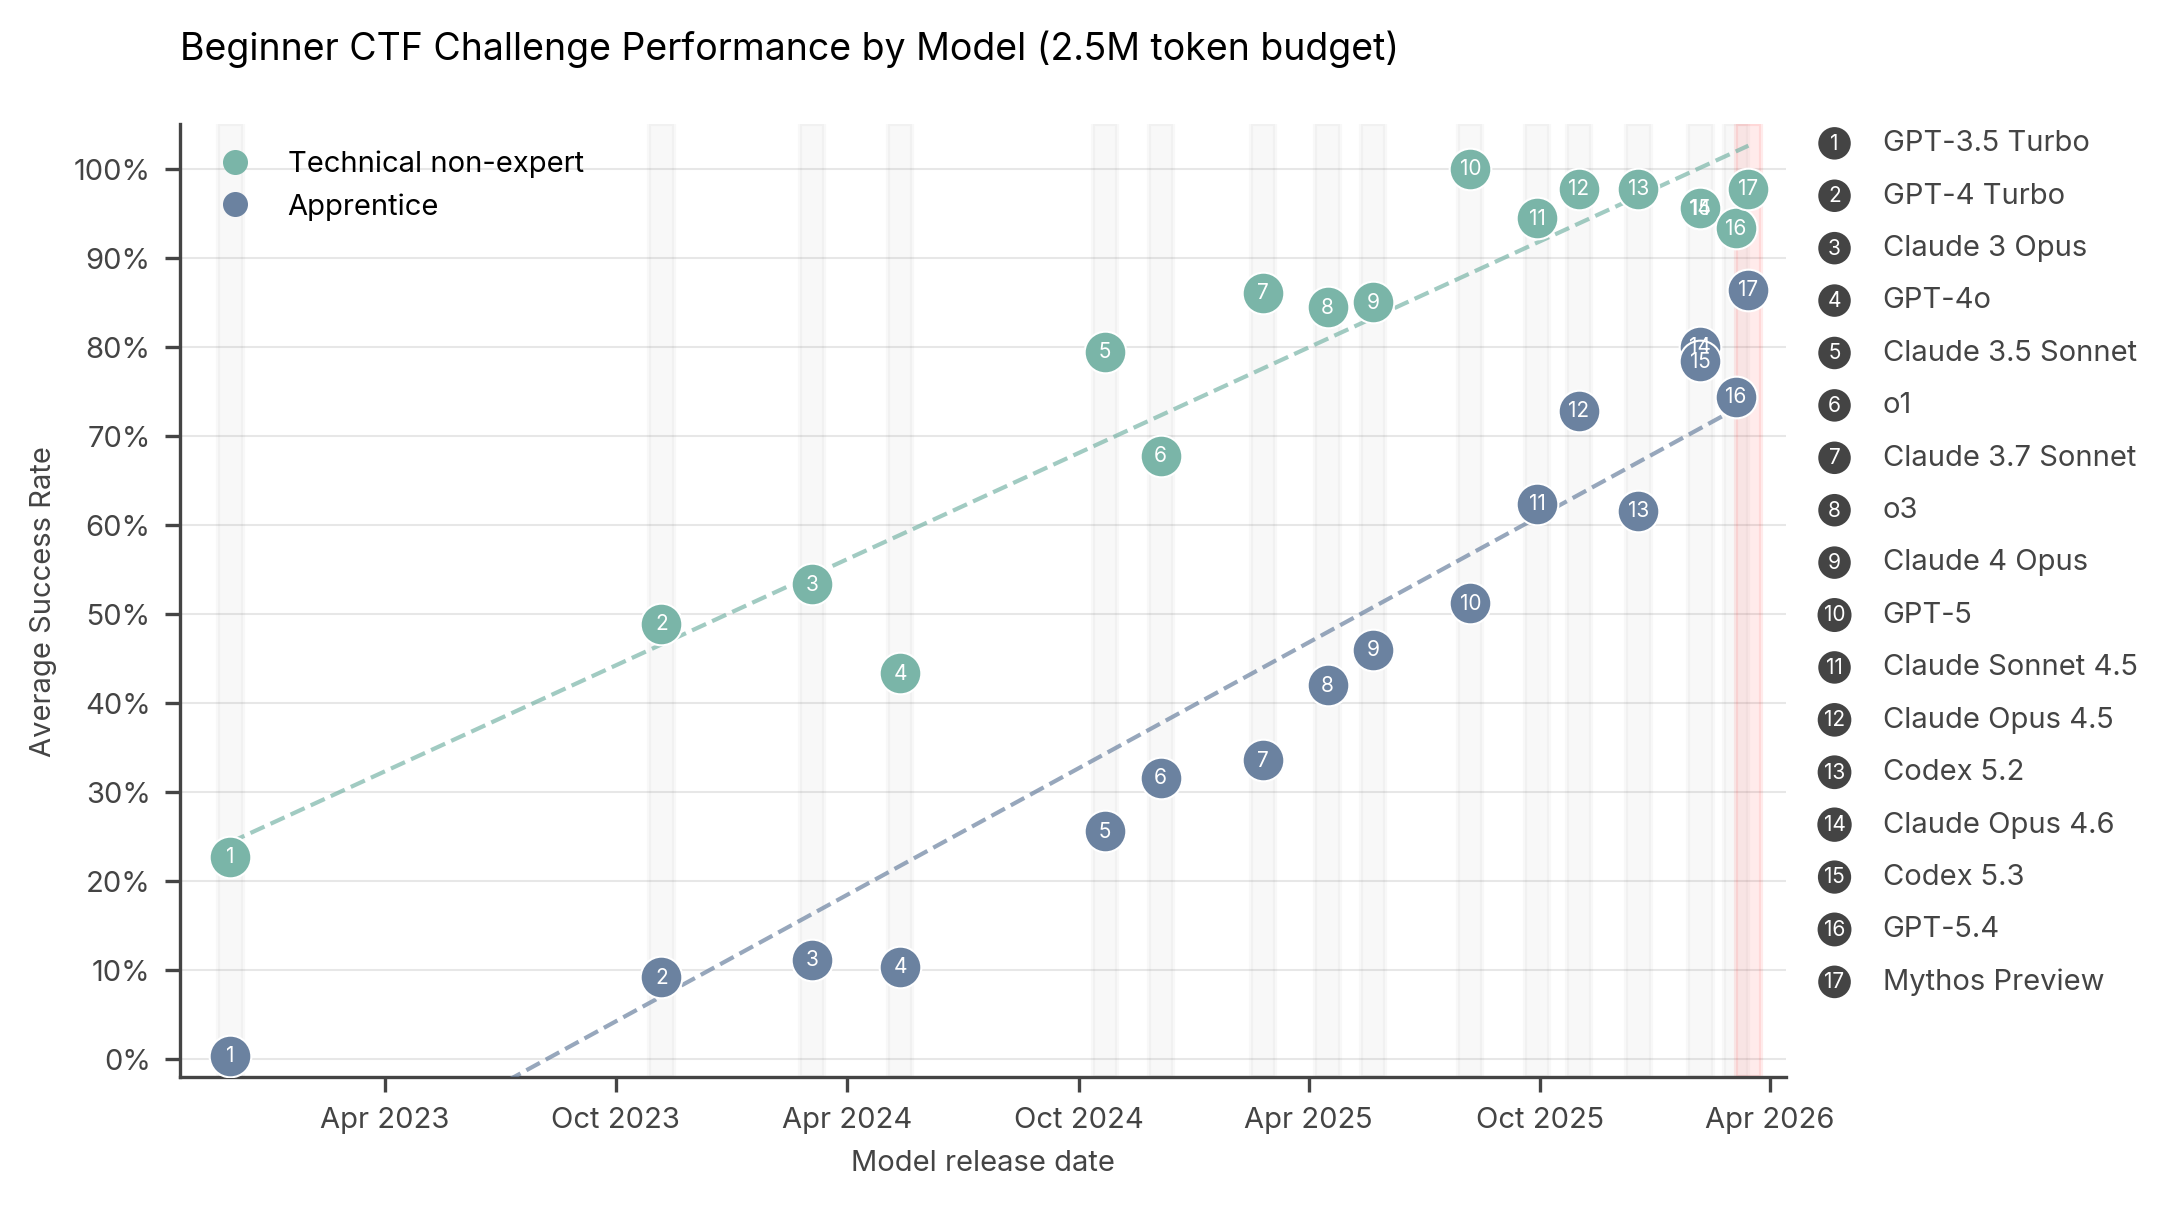
\includegraphics[width=\columnwidth]{ctf_nonexpert.png}
\caption{Performance auf \emph{non-expert} und \emph{apprentice} CTF-Aufgaben für Modelle seit November 2022. Quelle: AISI~\cite{aisi_claude_mythos_2026}.}
\label{fig:ctf_nonexpert}
\end{figure}

Auf den höheren Schwierigkeitsstufen \emph{practitioner} und \emph{expert} (Abbildung~\ref{fig:ctf_expert}) wird der Abstand sichtbarer, bleibt aber moderat: Mythos löst hier rund 73\,\% der Aufgaben, während die stärksten öffentlichen Modelle nur etwa 5\,Prozentpunkte darunter liegen und in einzelnen Kategorien ebenfalls auf gleichem Niveau abschneiden~\cite{aisi_claude_mythos_2026}.

\begin{figure}[!htbp]
\centering
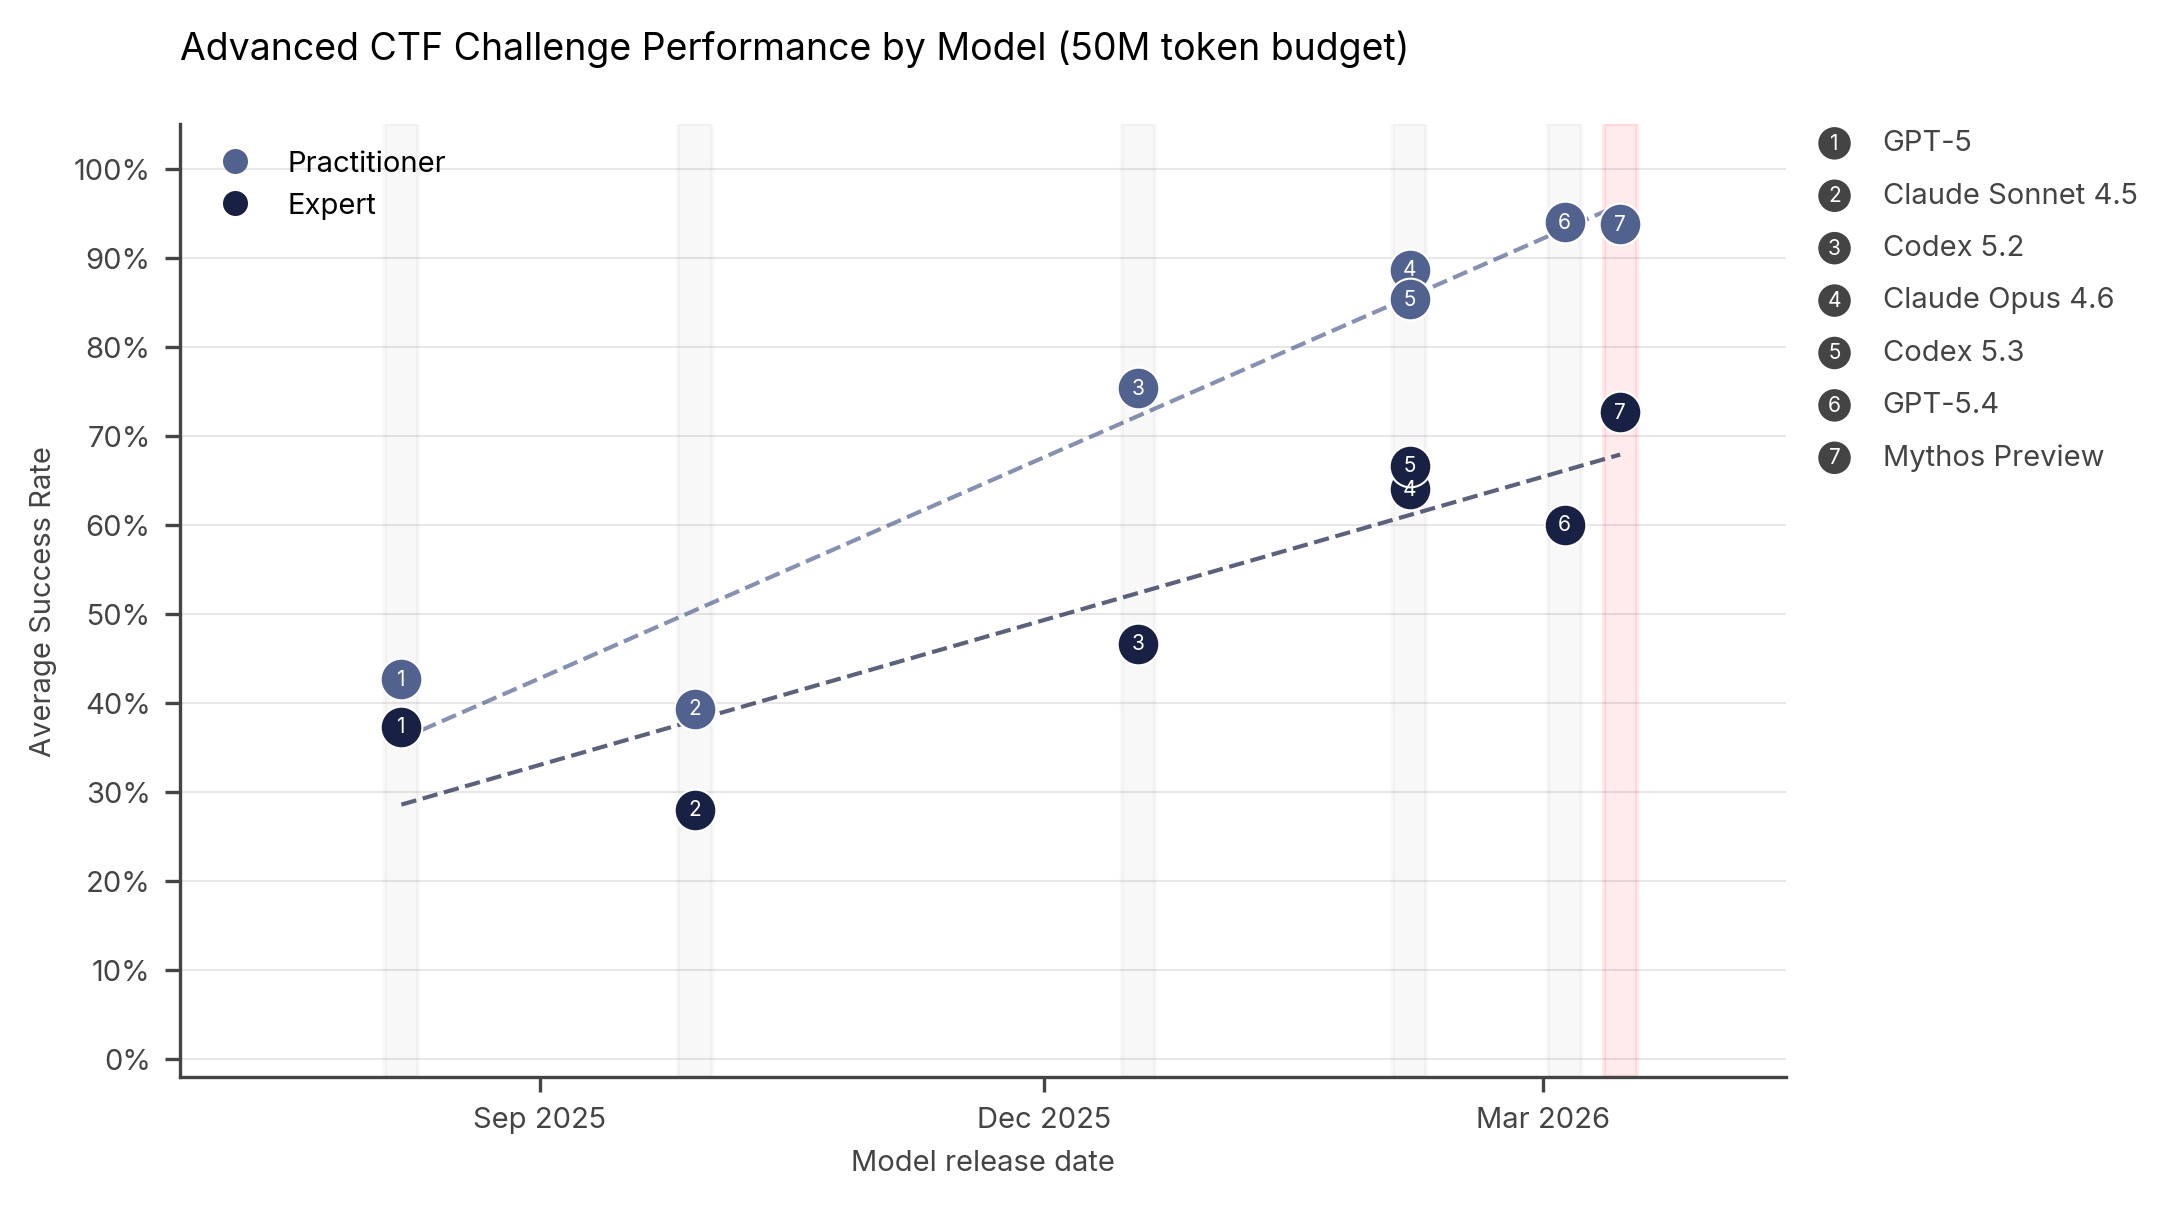
\includegraphics[width=\columnwidth]{ctf_expert.png}
\caption{Performance auf \emph{practitioner} und \emph{expert} CTF-Aufgaben für Modelle seit August 2025. Quelle: AISI~\cite{aisi_claude_mythos_2026}.}
\label{fig:ctf_expert}
\end{figure}

Daraus ergibt sich eine Beobachtung: Mythos definiert zwar den aktuellen Stand der Technik im Bereich offensiver KI-Fähigkeiten, der Abstand zur breit verfügbaren Modellbasis ist jedoch klein. Schon ein Leistungsdelta von rund 5\,Prozentpunkten auf Expert-Level-CTFs bedeutet, dass die in den folgenden Abschnitten diskutierten Angriffsvektoren nicht auf Mythos beschränkt sind, sondern in abgeschwächter Form bereits mit öffentlich zugänglichen Modellen realisiert werden können.

Diese Einschätzung wird durch eine unabhängige Reproduktionsstudie der Vidoc Security Labs gestützt~\cite{vidoc_mythos_reproduction_2026}. Vidoc hat die von Anthropic für Mythos berichteten Code-Schwachstellenfunde mit den öffentlich verfügbaren Modellen Claude Opus 4.6 und GPT-5.4 nachzustellen versucht und dabei in mehreren Kategorien identische Ergebnisse erzielt. Tabelle~\ref{tab:vidoc_repro} fasst die Befunde zusammen.

\begin{table}[!htbp]
\renewcommand{\arraystretch}{1.2}
\caption{Reproduktion der Mythos-Schwachstellenfunde mit öffentlichen Modellen. Quelle: Vidoc Security~\cite{vidoc_mythos_reproduction_2026}.}
\label{tab:vidoc_repro}
\centering
\footnotesize
\begin{tabular}{|l|l|l|}
\hline
\textbf{Ziel} & \textbf{Claude Opus 4.6} & \textbf{GPT-5.4} \\
\hline
FreeBSD (CVE-2026-4747) & exact (3/3) & exact (3/3) \\
\hline
OpenBSD (27-J.-Bug) & exact (3/3) & keine (0/3) \\
\hline
Botan (CVE-2026-34580/82) & exact (3/3) & exact (3/3) \\
\hline
FFmpeg (\texttt{h264\_slice.c}) & partial (3/3) & partial (3/3) \\
\hline
wolfSSL (CVE-2026-5194) & partial (3/3) & partial (3/3) \\
\hline
\end{tabular}
\end{table}

Vidoc berichtet, dass die Kosten für einen vollständigen Scan einer einzelnen Datei mit öffentlichen Modellen unter 30\,\$ blieben~\cite{vidoc_mythos_reproduction_2026}. Vor diesem Hintergrund ist auch die Preisstruktur der drei verglichenen Modelle aufschlussreich (Tabelle~\ref{tab:pricing}). Mythos ist je 1\,Mio.~Tokens deutlich teurer als die öffentlichen Alternativen.

\begin{table}[!htbp]
\renewcommand{\arraystretch}{1.2}
\caption{API-Preise je 1\,Mio.~Tokens (Stand: Juni 2026).}
\label{tab:pricing}
\centering
\footnotesize
\begin{tabular}{|l|r|r|}
\hline
\textbf{Modell} & \textbf{Input / 1M} & \textbf{Output / 1M} \\
\hline
GPT-5.4 & \$2{,}50 & \$15{,}00 \\
\hline
Claude Opus 4.6 & \$5{,}00 & \$25{,}00 \\
\hline
Claude Mythos & \$25{,}00 & \$125{,}00 \\
\hline
\end{tabular}
% TODO: Quellen f\"ur Preise ergänzen (Anthropic-Preisseite, OpenAI-Preisseite)
\end{table}

Aus der Kombination der CTF-Benchmarks, der Vidoc-Reproduktion und der Preisstruktur ergibt sich das Fazit des Vergleichs:
\begin{itemize}
  \item Öffentliche Modelle erzielen vergleichbare Schwachstellenfunde wie Mythos zu Kosten unter 30\,\$ pro Datei~\cite{vidoc_mythos_reproduction_2026}.
  \item Mythos ist in einzelnen Disziplinen weiterhin überlegen, stellt aber kein exklusives Werkzeug mehr dar, sondern markiert lediglich die obere Kante eines breit zugänglichen Spektrums.
  \item Der verbleibende Vorteil von Mythos liegt weniger im reinen Modell, sondern im umgebenden Tooling -- Agenten-Schleifen, Code-Ausführung und integrierten Recherche-Werkzeugen.
\end{itemize}

\section{Angriffsvektoren}
Der bisherige Vergleich konzentrierte sich primär auf die Disziplin der Code-Schwachstellenanalyse, in der sich der Abstand zwischen Mythos und öffentlichen Modellen als gering erwies. Diese ist jedoch nur ein Teilbereich des offensiven KI-Einsatzes. Über die reine Quellcode-Analyse hinaus existieren weitere Angriffsvektoren, in denen generative Modelle bestehende Angriffsmuster nicht nur beschleunigen, sondern qualitativ verändern. Die folgenden Abschnitte behandeln die drei relevantesten: Phishing \& Social Engineering, Code-Schwachstellenanalyse \& Exploit-Generierung sowie physische Schwachstellenanalyse \& Exploit-Generierung.

\subsection{Phishing \& Social Engineering}
Phishing und Social Engineering zählen seit Jahren zu den erfolgreichsten Einstiegsvektoren in Unternehmensnetzwerke. Generative KI verändert beide Felder grundlegend, weil sie bisherige Erkennungsmerkmale -- fehlerhafte Grammatik, unpersönliche Ansprache, holprige Übersetzungen -- weitgehend eliminiert und gleichzeitig die Skalierbarkeit hochgradig personalisierter Angriffe ermöglicht~\cite{hazell_spear_2023,_social_2025}.
\newline
\newline
\textbf{Phishing und Spear-Phishing}
\newline
Klassische Massen-Phishing-Kampagnen sind in der Vergangenheit häufig an der Sprachqualität gescheitert. Mit Large Language Models lassen sich Mails grammatisch einwandfrei und stilistisch glaubwürdig in nahezu jeder Sprache erzeugen, ohne dass der Angreifer diese selbst beherrschen muss. Studien zeigen, dass solche NLM-generierten Mails eine hohe Erfolgsquote aufweisen und für klassische Spam-Filter schwer zu detektieren sind~\cite{karanjai_targeted_2023}. In Kombination mit etablierten Phishing-Frameworks wie GoPhish oder King Phisher lassen sich KI-generierte Templates automatisiert an tausende Empfänger ausspielen. Hinzu kommen spezialisierte, unzensierte Modelle wie WormGPT und FraudGPT, die explizit für die Erstellung betrügerischer Inhalte beworben und in einschlägigen Foren gehandelt werden.
\newline % TODO: Quelle für WormGPT/FraudGPT ergänzen

Besonders kritisch ist die Verschiebung von breit gestreutem Phishing zu KI-skaliertem Spear-Phishing. Open-Source-Intelligence-Werkzeuge wie theHarvester, Maltego und SpiderFoot aggregieren öffentlich verfügbare Daten über Zielpersonen aus sozialen Netzwerken, Domain-Registries und Datenleaks. LLMs konsumieren diese Profile und erzeugen daraus individuell zugeschnittene Nachrichten. Hazell demonstriert dies an einer Kampagne gegen über 600 britische Parlamentsabgeordnete, bei der jede personalisierte Mail nur einen Bruchteil eines Cents kostet und Sicherheitsmechanismen heutiger LLMs durch einfaches Prompt-Engineering umgangen werden können~\cite{hazell_spear_2023}. Eine vergleichende Studie an rund 9.000 Beschäftigten einer großen Universität zeigt zudem, dass auch laterales Phishing aus kompromittierten internen Konten durch LLMs ebenso wirksam ist wie von Kommunikationsprofis verfasste Mails -- bei zeitkritischen Anlässen übertrifft die LLM-Variante die menschliche sogar~\cite{bethany_lateral_2025}.
\newline

Über die reine Textgenerierung hinaus werden gefälschte Login-Seiten zunehmend mit überzeugenden Begleit-Mails kombiniert. Adversary-in-the-Middle-Frameworks wie Evilginx sowie skript-basierte Werkzeuge wie Zphisher oder das Social Engineering Toolkit (SET) liefern die technische Infrastruktur zum Abgreifen von Session-Cookies und Zwei-Faktor-Token. Die LLM-gestützte Komponente liefert dazu kontextuell passende Tarnnachrichten, etwa vorgetäuschte IT-Tickets oder HR-Korrespondenz, die zur Eingabe der Zugangsdaten verleiten.
\newline
\newline
\textbf{Social Engineering}
\newline
Im klassischen Social-Engineering-Bereich verschärft sich die Lage durch generative Audio- und Videomodelle. Voice-Cloning-Dienste wie ElevenLabs ermöglichen die Synthese überzeugender Sprachnachrichten aus wenigen Sekunden Audiomaterial, das häufig aus öffentlich zugänglichen Videos, Podcasts oder Voicemails gewonnen wird. Praktische Untersuchungen zu KI-gestütztem Vishing demonstrieren die Machbarkeit solcher Angriffe unter realistischen Bedingungen~\cite{toapanta_aidriven_2024}. Auch Echtzeit-Videoanruf-Manipulationen mittels Deepfake-Tools wie DeepFaceLive werden in CEO-Fraud-Szenarien eingesetzt; Jampani beschreibt diese Entwicklung von einfachen Imitationen hin zu nahezu photorealistischen Repliken realer Stimmen und Gesichter und verweist insbesondere auf die hohen finanziellen Schäden in den Sektoren Finanzwesen und Gesundheit~\cite{_social_2025}. % TODO: dokumentierte Einzelfälle

Eine weitere Angriffsvektor ist die Chat-Impersonation. LLMs können den Schreibstil einer Person aus wenigen Beispielnachrichten replizieren und in laufenden Konversationen über Messenger-Plattformen oder Kollaborationstools die Identität eines Kollegen oder Vorgesetzten übernehmen. % TODO: Quelle f\"ur Chat-Impersonation / Stilklonung ergänzen
Da viele Authentifizierungsprozesse weiterhin auf vertrauten Kommunikationskanälen und stilistischer Wiedererkennung beruhen, verlieren diese Heuristiken ihre Schutzwirkung. Damit verschwimmt die Grenze zwischen technischem Angriff und sozialer Manipulation zunehmend, und etablierte Verifikationsmechanismen wie Rückruf oder Out-of-Band-Bestätigung gewinnen an Bedeutung.

\subsection{Code Schwachstellenanalyse \& Exploit generierung}
Wo Social Engineering den menschlichen Faktor als Einstiegspunkt ausnutzt, richtet sich der zweite Angriffsvektor unmittelbar gegen das technische Substrat: den Quellcode und die Binärdateien hinter digitalen Systemen. Generative KI-Modelle ermöglichen es Angreifern, Codebasen in einem Umfang und einer Geschwindigkeit zu durchsuchen, die manueller Analyse bislang unzugänglich waren -- ohne dass tiefes Expertenwissen in statischer Analyse oder Reverse Engineering vorausgesetzt werden muss.
\newline
\newline
\textbf{Tools}
\newline
Für die KI-gestützte Schwachstellenanalyse steht Angreifern ein zweigliedriges Werkzeugspektrum zur Verfügung. Spezialisierte, ungefilterte Modelle wie WormGPT, FraudGPT und GhostGPT werden explizit ohne Sicherheitsschranken betrieben und sind auf offensive Anwendungsfälle ausgelegt. Als Alternative bieten selbst-gehostete Open-Source-Modelle wie Qwen, betrieben über Frameworks wie Ollama, vollständige Kontrolle über jede Sicherheitsschicht -- und damit die Möglichkeit, diese vollständig zu entfernen.
\newline

Öffentlich verfügbare Frontier-Modelle wie Claude, GPT oder Gemini lassen sich durch Jailbreak-Techniken für offensive Zwecke nutzbar machen. DrAttack demonstriert exemplarisch, wie Prompt-Dekomposition und -Rekonstruktion die Sicherheitsfilter dieser Modelle systematisch aushebeln: Schädliche Anfragen werden in harmlos wirkende Teilprompts zerlegt, getrennt an das Modell übermittelt und anschließend zur ursprünglichen Exploit-Anfrage zusammengeführt~\cite{li_drattack_2024}. Diese Technik ist paradigmatisch für eine breite Klasse von Jailbreak-Methoden, die unter dem Begriff DAN (Do Anything Now) zusammengefasst werden und die inhärenten Sicherheitsbeschränkungen öffentlicher Modelle durch strukturelle Prompt-Manipulation umgehen.
\newline
\newline
\textbf{Anwendungsfälle}
\newline
Das Einsatzspektrum reicht von der Analyse von Web-Frontends bis zum Reverse Engineering nativer Binärdateien. Im Web-Kontext lassen sich LLMs einsetzen, um JavaScript-Code auf clientseitige Schwachstellen -- unsichere DOM-Manipulationen, unsanitisierte Eingaben oder exponierte API-Schlüssel -- zu untersuchen und darauf aufbauend gezielt manipulierten Code zu erzeugen, der diese Lücken ausnutzt.
\newline

Besonders wirkungsvoll für die strukturierte Schwachstellensuche in großen Codebasen ist der IRIS-Ansatz~\cite{li_iris_2024}. IRIS kombiniert LLM-gestützte semantische Analyse mit klassischer statischer Programmanalyse, um sicherheitsrelevante Schwachstellen in umfangreichen Open-Source-Projekten wie dem Linux-Kernel oder Firefox zu identifizieren. Das Sprachmodell kompensiert dabei die strukturellen Schwächen regelbasierter Analyzer -- fehlende Kontextsensitivität und hohe Falsch-Positiv-Raten -- indem es semantische Zusammenhänge über Funktionsgrenzen hinweg versteht. Aus Angreiferperspektive lässt sich derselbe Ansatz offensiv wenden: Wer identifizierte Schwachstellen nicht meldet, sondern zu funktionsfähigen Exploits weiterentwickelt, gewinnt einen erheblichen Informationsvorsprung gegenüber den Maintainern betroffener Projekte.
\newline

Im Bereich des Reverse Engineering ermöglicht KI schließlich die Analyse von Binärdateien ohne vorliegenden Quellcode. LLMs können dekompilierten Code aus Werkzeugen wie Ghidra oder IDA Pro semantisch interpretieren und auf Speicherfehler, Use-after-free-Muster oder Integer-Overflows hinweisen -- ohne dass der Angreifer die Rohdekompilierung manuell auswerten muss. Die Kombination aus automatisierter Dekompilierung und KI-gestützter Interpretation senkt die Einstiegshürde für die Analyse proprietärer Software erheblich und macht bislang spezialisierten Fachkräften vorbehaltene Angriffsflächen einem breiteren Täterkreis zugänglich.

\subsection{Physische Schwachstellenanalyse \& Exploit generierung}

\section{OWASP-Jucieshop Code-analyse \label{cha:demo}} 

\section{Fazit}
Durch den einsatz von KI Hilfsmittelen von Angreifern ist es leichter Schwachstellen zu finden und diese auszunutzen. Gerade im Bereich Phishing und Socialengineering macht der gebrauch einer LLM vieles einfacher und schneller. Um eine gute qualität zu erhalten ist kein Top Modell erfoderlich, wie z.B. bei der Schwachstellenanalyse. Da Software immer sicherer wird und die meisten Angrife durch Phishing oder Socialengineering gestartet werden, senkt ein LLM diese Hürde noch weiter. Trotzdem ändert ein LLM nicht unbedingt den Ablauf sondern vereinfach nur Schritte, wie das übersetzen. Die Gefahr steigt für Privat Personen mehr and als für Firmen. Da im Privatenbereich nicht so viele Schutzmechanismen existieren wie im Enterprisebereich.

Die interessanteren Angriffsvektoren sind die Schwachstellenanalyse von . 
Unter betrachtung der Ergebnisse aus Kapitel \ref{cha:mythosvsoffentlich} und dem eigenem Versuch im Kapitel \ref{cha:demo}. Daraus kann abgeleitet werden das die Ergebnisse von Mythos eine bessere Qualität haben. Die Schwachstellen könnnen auch mit öffentlich zugänglichen Modellen gefunden und ausgenutzt werden, die Qualität und konsetenz ist nicht so sicher wie bei Mythos.







\section*{Acknowledgment}


The authors would like to thank...






\bibliographystyle{bibtex/IEEEtran}
\bibliography{bibtex/Quellen}




\end{document}


%
% paper title
% Titles are generally capitalized except for words such as a, an, and, as,
% at, but, by, for, in, nor, of, on, or, the, to and up, which are usually
% not capitalized unless they are the first or last word of the title.
% Linebreaks \\ can be used within to get better formatting as desired.
% Do not put math or special symbols in the title.

% An example of a floating figure using the graphicx package.
% Note that \label must occur AFTER (or within) \caption.
% For figures, \caption should occur after the \includegraphics.
% Note that IEEEtran v1.7 and later has special internal code that
% is designed to preserve the operation of \label within \caption
% even when the captionsoff option is in effect. However, because
% of issues like this, it may be the safest practice to put all your
% \label just after \caption rather than within \caption{}.
%
% Reminder: the "draftcls" or "draftclsnofoot", not "draft", class
% option should be used if it is desired that the figures are to be
% displayed while in draft mode.
%
%\begin{figure}[!t]
%\centering
%\includegraphics[width=2.5in]{myfigure}
% where an .eps filename suffix will be assumed under latex, 
% and a .pdf suffix will be assumed for pdflatex; or what has been declared
% via \DeclareGraphicsExtensions.
%\caption{Simulation results for the network.}
%\label{fig_sim}
%\end{figure}

% Note that the IEEE typically puts floats only at the top, even when this
% results in a large percentage of a column being occupied by floats.


% An example of a double column floating figure using two subfigures.
% (The subfig.sty package must be loaded for this to work.)
% The subfigure \label commands are set within each subfloat command,
% and the \label for the overall figure must come after \caption.
% \hfil is used as a separator to get equal spacing.
% Watch out that the combined width of all the subfigures on a 
% line do not exceed the text width or a line break will occur.
%
%\begin{figure*}[!t]
%\centering
%\subfloat[Case I]{\includegraphics[width=2.5in]{box}%
%\label{fig_first_case}}
%\hfil
%\subfloat[Case II]{\includegraphics[width=2.5in]{box}%
%\label{fig_second_case}}
%\caption{Simulation results for the network.}
%\label{fig_sim}
%\end{figure*}
%
% Note that often IEEE papers with subfigures do not employ subfigure
% captions (using the optional argument to \subfloat[]), but instead will
% reference/describe all of them (a), (b), etc., within the main caption.
% Be aware that for subfig.sty to generate the (a), (b), etc., subfigure
% labels, the optional argument to \subfloat must be present. If a
% subcaption is not desired, just leave its contents blank,
% e.g., \subfloat[].


% An example of a floating table. Note that, for IEEE style tables, the
% \caption command should come BEFORE the table and, given that table
% captions serve much like titles, are usually capitalized except for words
% such as a, an, and, as, at, but, by, for, in, nor, of, on, or, the, to
% and up, which are usually not capitalized unless they are the first or
% last word of the caption. Table text will default to \footnotesize as
% the IEEE normally uses this smaller font for tables.
% The \label must come after \caption as always.
%
%\begin{table}[!t]
%% increase table row spacing, adjust to taste
%\renewcommand{\arraystretch}{1.3}
% if using array.sty, it might be a good idea to tweak the value of
% \extrarowheight as needed to properly center the text within the cells
%\caption{An Example of a Table}
%\label{table_example}
%\centering
%% Some packages, such as MDW tools, offer better commands for making tables
%% than the plain LaTeX2e tabular which is used here.
%\begin{tabular}{|c||c|}
%\hline
%One & Two\\
%\hline
%Three & Four\\
%\hline
%\end{tabular}
%\end{table}


% Note that the IEEE does not put floats in the very first column
% - or typically anywhere on the first page for that matter. Also,
% in-text middle ("here") positioning is typically not used, but it
% is allowed and encouraged for Computer Society conferences (but
% not Computer Society journals). Most IEEE journals/conferences use
% top floats exclusively. 
% Note that, LaTeX2e, unlike IEEE journals/conferences, places
% footnotes above bottom floats. This can be corrected via the
% \fnbelowfloat command of the stfloats package.


% trigger a \newpage just before the given reference
% number - used to balance the columns on the last page
% adjust value as needed - may need to be readjusted if
% the document is modified later
%\IEEEtriggeratref{8}
% The "triggered" command can be changed if desired:
%\IEEEtriggercmd{\enlargethispage{-5in}}

% references section

% can use a bibliography generated by BibTeX as a .bbl file
% BibTeX documentation can be easily obtained at:
% http://mirror.ctan.org/biblio/bibtex/contrib/doc/
% The IEEEtran BibTeX style support page is at:
% http://www.michaelshell.org/tex/ieeetran/bibtex/

% *** CITATION PACKAGES ***
%
%\usepackage{cite}
% cite.sty was written by Donald Arseneau
% V1.6 and later of IEEEtran pre-defines the format of the cite.sty package
% \cite{} output to follow that of the IEEE. Loading the cite package will
% result in citation numbers being automatically sorted and properly
% "compressed/ranged". e.g., [1], [9], [2], [7], [5], [6] without using
% cite.sty will become [1], [2], [5]--[7], [9] using cite.sty. cite.sty's
% \cite will automatically add leading space, if needed. Use cite.sty's
% noadjust option (cite.sty V3.8 and later) if you want to turn this off
% such as if a citation ever needs to be enclosed in parenthesis.
% cite.sty is already installed on most LaTeX systems. Be sure and use
% version 5.0 (2009-03-20) and later if using hyperref.sty.
% The latest version can be obtained at:
% http://www.ctan.org/pkg/cite
% The documentation is contained in the cite.sty file itself.





% graphicx was written by David Carlisle and Sebastian Rahtz. It is
% required if you want graphics, photos, etc. graphicx.sty is already
% installed on most LaTeX systems. The latest version and documentation
% can be obtained at: 
% http://www.ctan.org/pkg/graphicx
% Another good source of documentation is "Using Imported Graphics in
% LaTeX2e" by Keith Reckdahl which can be found at:
% http://www.ctan.org/pkg/epslatex
%
% latex, and pdflatex in dvi mode, support graphics in encapsulated
% postscript (.eps) format. pdflatex in pdf mode supports graphics
% in .pdf, .jpeg, .png and .mps (metapost) formats. Users should ensure
% that all non-photo figures use a vector format (.eps, .pdf, .mps) and
% not a bitmapped formats (.jpeg, .png). The IEEE frowns on bitmapped formats
% which can result in "jaggedy"/blurry rendering of lines and letters as
% well as large increases in file sizes.
%
% You can find documentation about the pdfTeX application at:
% http://www.tug.org/applications/pdftex





% *** MATH PACKAGES ***
%
%\usepackage{amsmath}
% A popular package from the American Mathematical Society that provides
% many useful and powerful commands for dealing with mathematics.
%
% Note that the amsmath package sets \interdisplaylinepenalty to 10000
% thus preventing page breaks from occurring within multiline equations. Use:
%\interdisplaylinepenalty=2500
% after loading amsmath to restore such page breaks as IEEEtran.cls normally
% does. amsmath.sty is already installed on most LaTeX systems. The latest
% version and documentation can be obtained at:
% http://www.ctan.org/pkg/amsmath





% *** SPECIALIZED LIST PACKAGES ***
%
%\usepackage{algorithmic}
% algorithmic.sty was written by Peter Williams and Rogerio Brito.
% This package provides an algorithmic environment fo describing algorithms.
% You can use the algorithmic environment in-text or within a figure
% environment to provide for a floating algorithm. Do NOT use the algorithm
% floating environment provided by algorithm.sty (by the same authors) or
% algorithm2e.sty (by Christophe Fiorio) as the IEEE does not use dedicated
% algorithm float types and packages that provide these will not provide
% correct IEEE style captions. The latest version and documentation of
% algorithmic.sty can be obtained at:
% http://www.ctan.org/pkg/algorithms
% Also of interest may be the (relatively newer and more customizable)
% algorithmicx.sty package by Szasz Janos:
% http://www.ctan.org/pkg/algorithmicx




% *** ALIGNMENT PACKAGES ***
%
%\usepackage{array}
% Frank Mittelbach's and David Carlisle's array.sty patches and improves
% the standard LaTeX2e array and tabular environments to provide better
% appearance and additional user controls. As the default LaTeX2e table
% generation code is lacking to the point of almost being broken with
% respect to the quality of the end results, all users are strongly
% advised to use an enhanced (at the very least that provided by array.sty)
% set of table tools. array.sty is already installed on most systems. The
% latest version and documentation can be obtained at:
% http://www.ctan.org/pkg/array


% IEEEtran contains the IEEEeqnarray family of commands that can be used to
% generate multiline equations as well as matrices, tables, etc., of high
% quality.




% *** SUBFIGURE PACKAGES ***
%\ifCLASSOPTIONcompsoc
%  \usepackage[caption=false,font=normalsize,labelfont=sf,textfont=sf]{subfig}
%\else
%  \usepackage[caption=false,font=footnotesize]{subfig}
%\fi
% subfig.sty, written by Steven Douglas Cochran, is the modern replacement
% for subfigure.sty, the latter of which is no longer maintained and is
% incompatible with some LaTeX packages including fixltx2e. However,
% subfig.sty requires and automatically loads Axel Sommerfeldt's caption.sty
% which will override IEEEtran.cls' handling of captions and this will result
% in non-IEEE style figure/table captions. To prevent this problem, be sure
% and invoke subfig.sty's "caption=false" package option (available since
% subfig.sty version 1.3, 2005/06/28) as this is will preserve IEEEtran.cls
% handling of captions.
% Note that the Computer Society format requires a larger sans serif font
% than the serif footnote size font used in traditional IEEE formatting
% and thus the need to invoke different subfig.sty package options depending
% on whether compsoc mode has been enabled.
%
% The latest version and documentation of subfig.sty can be obtained at:
% http://www.ctan.org/pkg/subfig




% *** FLOAT PACKAGES ***
%
%\usepackage{fixltx2e}
% fixltx2e, the successor to the earlier fix2col.sty, was written by
% Frank Mittelbach and David Carlisle. This package corrects a few problems
% in the LaTeX2e kernel, the most notable of which is that in current
% LaTeX2e releases, the ordering of single and double column floats is not
% guaranteed to be preserved. Thus, an unpatched LaTeX2e can allow a
% single column figure to be placed prior to an earlier double column
% figure.
% Be aware that LaTeX2e kernels dated 2015 and later have fixltx2e.sty's
% corrections already built into the system in which case a warning will
% be issued if an attempt is made to load fixltx2e.sty as it is no longer
% needed.
% The latest version and documentation can be found at:
% http://www.ctan.org/pkg/fixltx2e


%\usepackage{stfloats}
% stfloats.sty was written by Sigitas Tolusis. This package gives LaTeX2e
% the ability to do double column floats at the bottom of the page as well
% as the top. (e.g., "\begin{figure*}[!b]" is not normally possible in
% LaTeX2e). It also provides a command:
%\fnbelowfloat
% to enable the placement of footnotes below bottom floats (the standard
% LaTeX2e kernel puts them above bottom floats). This is an invasive package
% which rewrites many portions of the LaTeX2e float routines. It may not work
% with other packages that modify the LaTeX2e float routines. The latest
% version and documentation can be obtained at:
% http://www.ctan.org/pkg/stfloats
% Do not use the stfloats baselinefloat ability as the IEEE does not allow
% \baselineskip to stretch. Authors submitting work to the IEEE should note
% that the IEEE rarely uses double column equations and that authors should try
% to avoid such use. Do not be tempted to use the cuted.sty or midfloat.sty
% packages (also by Sigitas Tolusis) as the IEEE does not format its papers in
% such ways.
% Do not attempt to use stfloats with fixltx2e as they are incompatible.
% Instead, use Morten Hogholm'a dblfloatfix which combines the features
% of both fixltx2e and stfloats:
%
% \usepackage{dblfloatfix}
% The latest version can be found at:
% http://www.ctan.org/pkg/dblfloatfix




% *** PDF, URL AND HYPERLINK PACKAGES ***
%
%\usepackage{url}
% url.sty was written by Donald Arseneau. It provides better support for
% handling and breaking URLs. url.sty is already installed on most LaTeX
% systems. The latest version and documentation can be obtained at:
% http://www.ctan.org/pkg/url
% Basically, \url{my_url_here}.
